\documentclass{report} 
\title{Signals And Systems by Alan V. Oppenheim:\\Notes}
\date{Started 17 April 2025}
\author{Malcolm}
\usepackage{amsmath} %import math
\usepackage{mathtools} %more math
\usepackage{amssymb} %for QED symbol
\usepackage{amsthm} %
\usepackage{bm}%bold math
\usepackage{graphicx} %import imaging
\graphicspath{{./images/}} %set imaging path
\begin{document}
\maketitle

\tableofcontents

\newpage
\section{Introduction}
\subsection{Signal Energy and Power}
\textbf{Motivation and definition}\\
In many but not all, applications, the signals considered directly related to physical quantities capturing
power and energy in a physical system. (for instance $v^2/R$ for the power across a resistor)\\
\vspace{1mm}\\
As such it is a common and worthwhile convention to use similar terminology for power and energy for \textit{any} 
continuous-time signal, denoted $x(t)$, or any discrete-time signal $x[n]$. 
In this case, the total energy over the time interval $t_1\leq t\leq t_2$ in a continuous signal $x(t)$ is defined
as
\begin{equation*}
\int^{t_2}_{t_1}|x(t)|^2dt
\end{equation*}
where $|x|$ denotes the magnitude of the (possibly complex) number $x$; see that the time-averaged signal 
can be obtained by dividing by $(t_2-t_1)$. Similarly for a discrete signal $x[n]$ over the interval $n_1\leq n\leq n_2$ the total energy is
\begin{equation*}
\sum^{n_2}_{n=n_1}|x[n]|^2
\end{equation*}
with the average power calculated by dividing by $(n_2-n_1+1)$.\\
\vspace{1mm}\\
It is important to remember that the terms `power' and `energy' are used here \textit{independently} of their 
relation to physical energy (they clearly don't correlate since their units or scalings would differ). Nevertheless
we will find it convenient to use these terms in a general fashion.\\
\vspace{1mm}\\
\textbf{Power and energy over infinite intervals}\\
Considering signals over an infinite time interval, meaning for $-\infty<t<+\infty$ or $-\infty<n<+\infty$. 
Here we define the total energy as the limits of the aforementioned equations increase without bound; in continuous
time,
\begin{equation*}
E_\infty\triangleq\lim_{T\to\infty}\int^T_{-T}|x(t)|^2dt
=\int^{+\infty}_{-\infty}|x(t)|^2dt
\end{equation*}
and in discrete time,
\begin{equation*}
E_\infty\triangleq\lim_{N\to\infty}\sum^{+N}_{n=-N}|x[n]|^2=\sum^{+\infty}_{n=-\infty}|x[n]|^2
\end{equation*}
Note that these expressions may not converge; for instance say $x(t)$ or $x[n]$ equal some nonzero constant for 
all time: such signals have infinite energy, while signals with $E_\infty<\infty$ have finite energy.\\
(next page)\newpage
\noindent\textbf{Cont.}\\
Analagously, we can define the time-averaged power over an infinite interval as
\begin{equation*}
P_\infty\triangleq\lim_{T\to\infty}\frac{1}{2T}\int^T_{-T}|x(t)|^2dt
\end{equation*}
and
\begin{equation*}
P_\infty\triangleq\lim_{N\to\infty}\frac{1}{2N+1}\sum^{+N}_{n=-N}|x[n]|^2
\end{equation*}
In continuous and discrete time respectively. \\
\vspace{1mm}\\
\textbf{Intuition}\\
See that with these definitions, we can identify three classes of signals: first those with finite total energy,
meaning $E_\infty<\infty$. See that such a signal would have zero average power:
\begin{equation*}
P_\infty=\lim_{T\to\infty}\frac{E_\infty}{2T}=0
\end{equation*}
Second would be signals with finite average power $P_\infty$; see from the above expression that for $P_\infty>0$,
this requires that $E_\infty=\infty$.\\
\vspace{1mm}\\
Last would be signals for which neither $P_\infty$ nor $E_\infty$ are finite. An example of this might be $x(t)=t$.\\
\vspace{1mm}\\
\textbf{Note on discrete signals}\\
It is omportant to note that the discrete-time signal $x[n]$ is defined \textit{only} for \textit{integer} 
values of the independent variable.
\newpage

\subsection{Even and Odd signals}
\textbf{Definition}\\
A continuous-time signal is \textit{even} if
\begin{equation*}
x(-t)=x(t)
\end{equation*}
while a discrete-time signal is \textit{even} if
\begin{equation*}
x[-n]=x[n]
\end{equation*}
These signals are referred to as \textit{odd} if
\begin{align*}
x(-t)&=-x(t)\\
x[-n]&=-x[n]
\end{align*}
Note that an odd signal must be 0 at $t=0$ or $n=0$ since the equations require that $x(0)=-x(0)$ and $x[0]=-x[0]$.
\\
\vspace{1mm}\\
\textbf{Decomposition}\\
An important fact is that any signal can be broken into a sum of two signals, where one is even and the other odd.
To see this, consider
\begin{equation*}
\text{Ev}\{x(t)\}=\frac{1}{2}[x(t)+x(-t)]
\end{equation*}
which is referred to as the \textit{even part} of $x(t)$. Similarly, the \textit{odd part} of $x(t)$ is given by
\begin{equation*}
\text{Od}\{x(t)\}=\frac{1}{2}[x(t)-x(-t)]
\end{equation*}
See that $x(t)$ is the sum of the two. Exactly analagous definitions hold in the discrete time case.
\begin{center}
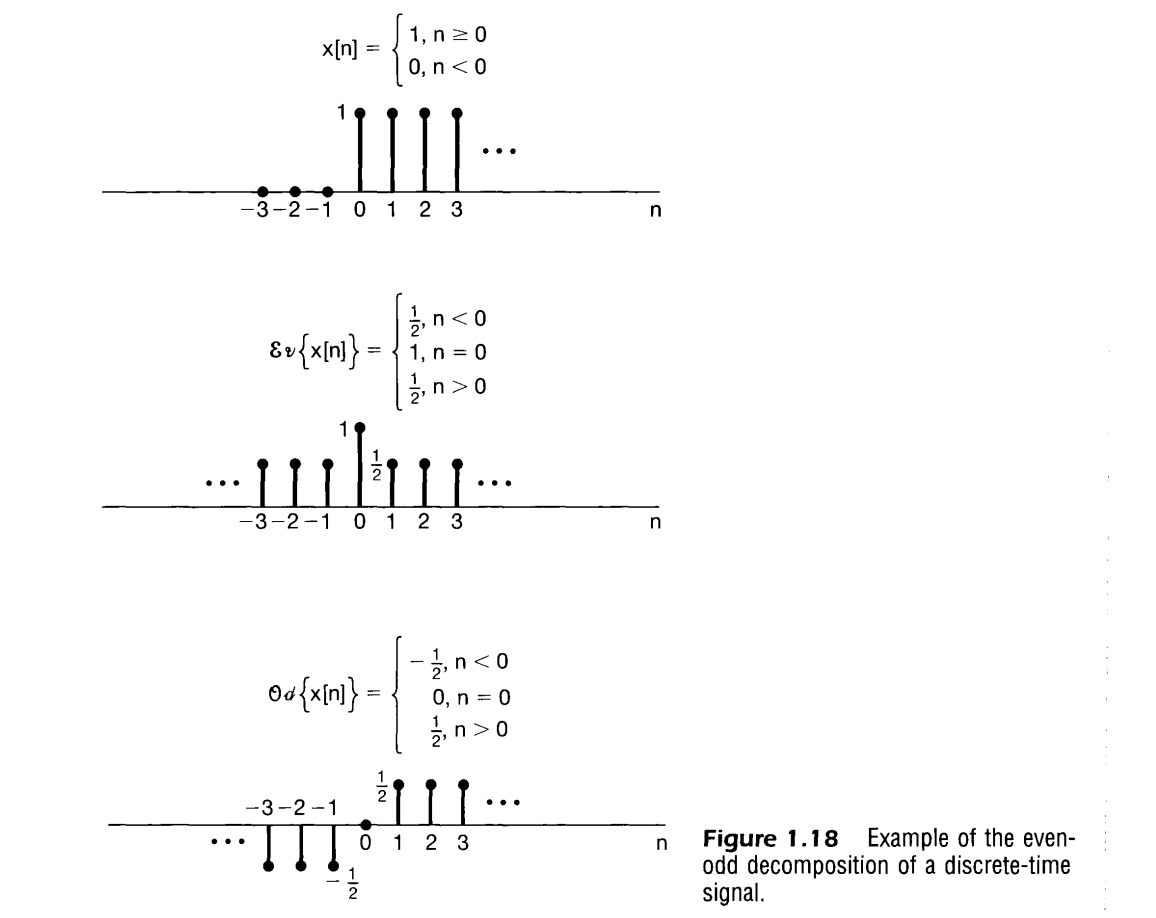
\includegraphics[width=9cm]{a1}
\end{center}
\newpage

\subsection{Differences between continuous and\\discrete periodic complex exponentials}
The continuous-time \textit{complex exponential signal} is of the form
\begin{equation*}
x(t)=Ce^{at}
\end{equation*}
where $C$ and $a$ are, in general, complex numbers. An important class of complex exponentials is obtained by constraining $a$ to be purely imaginary:
\begin{equation*}
x(t)=e^{i\omega t}
\end{equation*}
\textbf{Periodicity and harmonic relations (purely imaginary power)}\\
An important property of this signal is that it is periodic; recall that $x(t)$ will be periodic with period $T$ if
\begin{equation*}
e^{i\omega t}=e^{i\omega(t+T)}
\end{equation*}
this means
\begin{equation*}
e^{i\omega(t+T)}=e^{i\omega t}e^{i\omega T}\implies
e^{i\omega T}=1
\end{equation*}
If $\omega=0$ then this is satisfied for any $T$. If $\omega\neq0$, see that the \textit{fundamental period} 
$T_0$ of $x(t)$---that is, the smallest positive value of $T$ for which this holds---is
\begin{equation*}
T_0=\frac{2\pi}{|\omega|}
\end{equation*}
(the signals $e^{i\omega 0t}$ and $e^{-i\omega t}$ have the same fundamental period)
Naturally, there is a set of exponentials periodic to a common period $T_0$. These are said to be
\textit{harmonically related} complex exponentials; the necessary condition they satisfy is
\begin{equation*}
e^{i\omega T_0}=1
\end{equation*}
which implies that
\begin{equation*}
\omega T_0=2\pi k,\quad k=0,\pm1,\pm2,\ldots
\end{equation*}
(next page)\newpage
\noindent\textbf{Cont.}\\
We had
\begin{equation*}
\omega T_0=2\pi k,\quad k=0,\pm1,\pm2,\ldots
\end{equation*}
if we define
\begin{equation*}
\omega_0=\frac{2\pi}{T_0}
\end{equation*}
this means that the harmonic frequencies $\omega$ must be integer multiples of $\omega_0$:
\begin{equation*}
\phi_k(t)=e^{ik\omega_0t},\quad k=0,\pm1,\pm2,\ldots
\end{equation*}
For $k=0$, $\phi_k(t)$ is a constant, while for any other value of $k$, $\phi_k(t)$ is periodic with fundamental 
frequency $|k|\omega_0$ and fundamental period
\begin{equation*}
\frac{2\pi}{|k|\omega_0}=\frac{T_0}{|k|}
\end{equation*}
Each $\phi_k(t)$ itself defines a fundamental frequency and a corresponding fundamental period. 
(see that $|k|\omega_0\cdot T_0/|k|=2\pi$, so this scaled down period is the corresponding period
for this scaled up frequency. Each frequency is unique, point here is that they are also periodic with $T_0$)\\
\vspace{1mm}\\
Note that the $k$th harmonic $\phi_k(t)$ is still periodic with $T_0$; it goes through exactly $|k|$ of its 
fundamental periods during any time interval of length $T_0$. (the term `harmonic' is consistent with its use in
music, where it refers to tones resulting from variations in acoustic pressure at frequencies that are integer
multiples of a fundamental frequency)\\
(next page)\newpage
\noindent\textbf{Discrete case}\\
As in continuous time, an important signal in discrete time is the \textit{complex exponential signal}, defined as
\begin{equation*}
x[n]=C\alpha^n
\end{equation*}
where $C$ and $\alpha$ are, in general, complex numbers. See that this could also be expressed as
\begin{equation*}
x[n]=Ce^{\beta n}
\end{equation*}
where $\alpha=e^\beta$. See that we can constrain $\beta$ to be purely imaginary:
\begin{equation*}
x[n]=e^{i\omega_0n}
\end{equation*}
\textbf{Periodicity properties of Discrete-time complex exponentials}\\
While there are many similarities between continuous and discrete-time signals, there are a number of important
differences. For the continuous time signal $e^{i\omega_0t}$, we know that
\begin{itemize}
\item The larger the magnitude of $\omega_0$, the higher the rate of oscillation of the signal
\item $e^{i\omega_0t}$ is periodic for any value of $\omega_0$
\end{itemize}
These properties are different in the discrete-time case.\\
\vspace{1mm}\\
Given the first property, consider the discrete-time complex exponential with frequency $\omega_0+2\pi$:
\begin{equation*}
e^{i(\omega_0+2\pi)n}=e^{i2\pi n}e^{i\omega_0n}=e^{i\omega_0n}
\end{equation*}
(see that this is a direct result of the fact that we iterate through discrete time as integers) 
The exponential at frequency $\omega_0+2\pi$ is the \textit{same} as that at frequency $\omega_0$. 
This is unlike the continuous-time case where each distinct $\omega_0$ represents a distinct signal.\\
\vspace{1mm}\\
In discrete time, the signal with frequency $\omega_0$ is identical to the signals with frequencies 
$\omega_0\pm2\pi,\omega_0\pm4\pi$, and so on. Therefore when considering discrete time complex exponentials, 
see that we need only consider a frequency interval of length $2\pi$ in which to choose $\omega_0$, such as 
$0\leq\omega_0<2\pi$ or $-\pi\leq\omega_0<\pi$.\\
\vspace{1mm}\\
Also see that because of this the discrete exponential 
$e^{i\omega_0n}$ does \textit{not} have a continually 
increasing rate of oscillation as $\omega_0$ increases in magnitude; the signals will oscillate faster until we 
reach $\omega_0=\pi$, after which the rate of oscillation decreases until we reach $\omega_0=2\pi$, at which 
the same constant sequence as $\omega_0=0$ is produced.\\
(next page)\newpage
\noindent\textbf{Cont.}\\
The second property we wish to consider concerns the periodicity of the discrete time complex exponential. In
order for the signal $e^{i\omega_0n}$ to be periodic with
period $N>0$ we must have
\begin{equation*}
e^{i\omega_0(n+N)}=e^{i\omega_0n}
\end{equation*}
or equivalently 
\begin{equation*}
e^{i\omega_0N}=1
\end{equation*}
For this to hold, $\omega_0N$ must be a multiple of $2\pi$. That is, there must be an integer $m$ such that
\begin{equation*}
\omega_0N=2\pi m
\end{equation*}
or equivalently
\begin{equation*}
\frac{\omega_0}{2\pi}=\frac{m}{N}
\end{equation*}
The signal $e^{i\omega_0n}$ is periodic if $\omega_0/2\pi$ is a rational number and is not periodic otherwise.\\
\vspace{1mm}\\
\textbf{Fundamental period}\\
Recall the idea of a \textit{fundamental period}; in this case it would mean the smallest $N$ such that 
$\omega_0N=2\pi m$ holds (this is unlike the continuous case where there is always some $T$ where $\omega_0T=2\pi$); see that this occurs when $m$ and $N$ do not have any factors in common.\\
\vspace{1mm}\\
See that from this we can derive a \textit{fundamental frequency} as
\begin{equation*}
\frac{2\pi}{N}=\frac{\omega_0}{m}
\end{equation*}
(see that this frequency is always equal or lower---intuitively, to have a different wave that completes one
oscillation in $N$ time, its frequency will either be equal or lower)\\
\vspace{1mm}\\
To summarize
\begin{center}
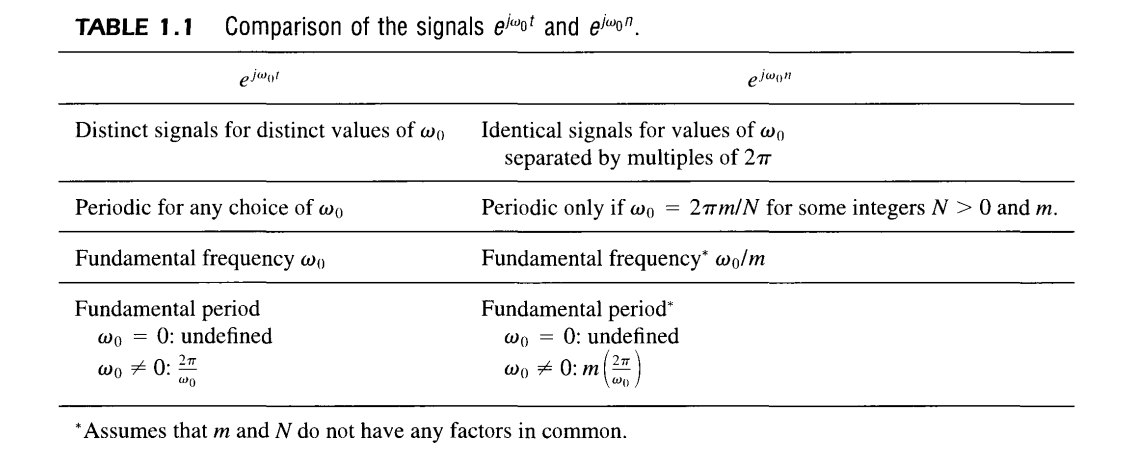
\includegraphics[width=10cm]{a2}
\end{center}
\newpage
\subsection{Intuition for discrete-time periodicity}
Consider the sequence $x[n]=\cos(2\pi n/12)$:
\begin{center}
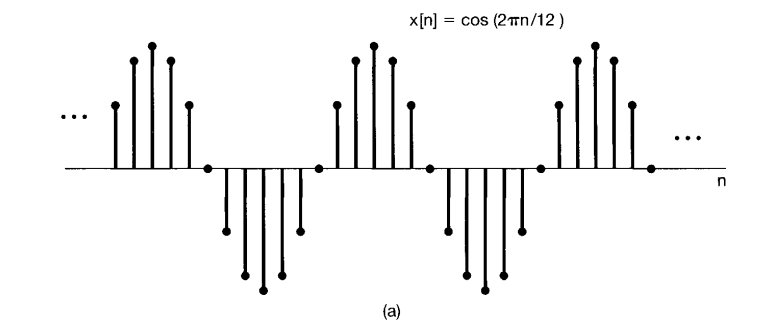
\includegraphics[width=10cm]{a3}
\end{center}
we can think of this as a set of samples of the continuous-time sinusoid $x(t)=\cos(2\pi t/12)$ at integer time
points. In this case, see that both $x(t)$ and $x[n]$ are periodic with fundamental period 12.
That is, the values of $x[n]$ repeat every 12 points, exactly in step with the fundamental period of $x(t)$.\\
\vspace{1mm}\\
Now consider the signal $x[n]=\cos(8\pi n/31)$:
\begin{center}
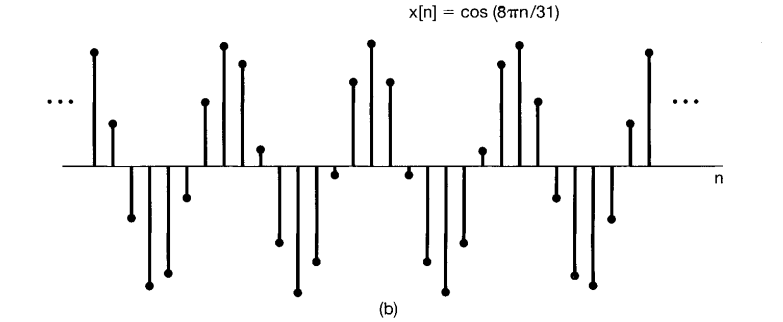
\includegraphics[width=10cm]{a4}
\end{center}
This can also be viewed as a set of samples of $x(t)=\cos(8\pi t/31)$ at integer points in time. 
But now see that in this case $x(t)$ is periodic with fundamental period $31/4$, while $x[n]$ is periodic with 
fundamental period 31.\\
\vspace{1mm}\\
This difference stems from the fact that the discrete-time signal is defined only for integer values of the 
independent variable---there is no sample at time
$t=31/4$, when $x(t)$ completes one period, or at $t=2\cdot31/4$ or $t=3\cdot31/4$, when $x(t)$ has completed two
or three periods. Only at sample $t=4\cdot31/4=31$, when
$x(t)$ has completed \textit{four} periods is the discrete sequence defined.\\
\vspace{1mm}\\
This manifests as the pattern of $x[n]$ not repeating with each cycle of positive and negative values, but rather
only after four of such cycles, specifically 31 points.
(next page)\newpage
\noindent\textbf{Cont.}\\
Finally consider



\newpage

\subsection{Difference in harmonic relations in discrete and\\continuous periodic exponentials}
















\end{document}
